\documentclass[12pt]{article}

\usepackage{graphicx}

\begin{document}

\title{PALFA Pipeline2.0 Documentation}
\author{Patrick Lazarus, Alex Samoilov, ... \\
        plazar@physics.mcgill.ca, alex@sequencefactory.com}
\date{\today}

\maketitle

\begin{abstract}
The PALFA Pipeline2.0 is an automated end-to-end pulsar search pipeline designed for the Pulsar-ALFA survey. The pipeline requests PALFA data from web services hosted at Cornell University, downloads data files, searches them, and finally uploads the results to the PALFA common database hosted at Cornell University.

The pipeline is written entirely in Python. It uses a SQLite database to track datafiles, and processing jobs. The pipeline is built around the \texttt{PRESTO} suite of pulsar search software. 

If you plan on using/modifying this pipeline to search data from other surveys please let me know.

\end{abstract}

\clearpage

\tableofcontents

\clearpage

\section{Features}
\begin{itemize}
    \item Sanity check of configurations
    \item Dynamic zapping
    \item Suite of tests to help initial set-up
    \item Automatic download of data files
    \item File size checks when downloading
    \item Notification of errors by email
    \item Automatic retry of failed jobs
    \item Results uploded are double-checked (i.e. database entries are compared with on-disk values)
    \item Results are uploaded as a single transaction, so no partial uploads when errors occur
    \item Automatic deletion of data files (upon success or terminal failure)
\end{itemize}

\section{Installation}
\subsection{Dependencies}
The PALFA pipeline has various dependencies. All of the following packages are required to run the pipeline.
\begin{itemize}
    \item PRESTO (a recent version is required. The new executable \texttt{fitsdelcol} must be included - https://github.com/scottransom/presto)
    \item psrfits\_utils (be sure to pull Kevin Stovall's version of psrfits\_utils. It contains the merging code required to analyse PALFA Mock spectrometer data. https://github.com/kstovall/psrfits\_utils.git)
    \item numpy (http://numpy.scipy.org/)
    \item M2Crypto (http://pypi.python.org/pypi/M2Crypto)
    \item PBSQuery (if PBS is being used - http://subtrac.sara.nl/oss/pbs\_python/wiki/TorqueInstallation)
    \item pyfits (http://www.stsci.edu/resources/software\_hardware/pyfits)
    \item pyodbc (http://pypi.python.org/pypi/pyodbc/)
    \item ImageMagick (on worker nodes - http://www.imagemagick.org/script/index.php)
    \item FreeTDS (required by pyodbc to connect to common-DB - http://www.freetds.org/)
    \item UnixODBC (required by pyodbc to connect to common-DB - http://www.unixodbc.org/)
    \item Drivers for ODBC - libtdsodbc.so and libmyodbc.so (In Debian these are available in the packages tdsodbc and libmyodbc, respectively).
    \item prettytable (http://code.google.com/p/prettytable/)
\end{itemize}

\textit{NOTE: Some of these dependencies have requirements of their own. For example, PRESTO requires cfitsio, TEMPO, numpy, scipy, etc. Be sure to follow the installation instructions for each packages.}

\subsection{Getting Started}
Here we will present basic step-by-step instructions for setting up the pipeline.

\begin{description}
    \item[Step 1] Create a directory where you want the pipeline to be installed.

    \item[Step 2] Download the pipeline source files. This should be done by cloning the git repository on github.com: https://github.com/plazar/pipeline2.0.

        \smallskip

        \texttt{\$ git clone git://github.com/plazar/pipeline2.0.git}

        \smallskip
        
        \textit{NOTE: This will create a sub-directory called ``pipeline2.0".} 

    \item[Step 3] Add the pipeline's lib/python directory to your PYTHONPATH environment variable. 

    \item[Step 4] For each of the example configuration files found in \texttt{lib/python/config/} make a copy with the same name, but with ``\_example'' removed. For example, \texttt{basic\_example.py} $\rightarrow$ \texttt{basic.py}. Next, for each of the newly created files modify the settings defined in it so they are appropriate for your system. It is possible to check the sanity of your configurations by executing the corresponding \texttt{*\_check.py} file. An error message will be displayed if a configuration is invalid. It is possible to rename all the example files at once using \texttt{awk}:

    \begin{verbatim}
        ls *_example.py | awk -F `_example' 
        `{printf(``cp %s %s%s\n'', $0, $1, $2)}' | sh
    \end{verbatim}

    \item[Step 5] Configure ODBC and FreeTDS. This can be done by editing the system-wide configuration files, or by creating the appropriate files (\texttt{.odbc.ini} and \texttt{.freetds.conf}, respectively) in your home area. See Section \ref{sec:dbconf} for details.

    \item[Step 6] Set up the job-tracker database. This is done using the script \texttt{bin/create\_database.py}. (Note that there are possibly some issues associated with accessing the job-tracker database over NFS. See Section \ref{sec:dbdetails} for details.)

    \item[Step 7] Perform tests. In the \texttt{tests/} directory there are some tests that can be run to see if you can connect to the common DB (\texttt{commondb\_test.py}), connect to the FTP server and data-restore webservice, use the e-mail system (\texttt{mailer\_test.py}), and FTP server (\texttt{cornellftp\_test.py}). There are also tests to check if the necessary python modules are available (\texttt{install\_test.py}), restore data (\texttt{restore\_test.py}), and submit jobs to the queue \texttt{submit\_test.py}. Note that the job-submission test executes \texttt{test\_job.py} on a worker node. This job checks for necessary software, and for the existence/permissions of directories. A report is printed to screen if there are errors. 
    
    To perform the tests call each script with the python interpreter. Additional information about the tests can be found in Section \ref{sec:tests}.

    \item[Step 8] Start the downloader using \texttt{StartDownloader.py}.
        
        \smallskip
        
        \textit{NOTE: The downloader does not need to be run on the same computer as the job pooler. However, the directory where the downloader saves files must be accessible from the computer where the job pooler is being run.}
        
        \smallskip
        
        Alternatively, it is possible to add files to the job-tracker database without using the downloader. To do this use \texttt{add\_files.py}. Be sure to set the \texttt{delete\_rawdata} configuration to \texttt{False} if you do not want raw data files to be deleted when the pipeline no longer requires them. 

    \item[Step 8] Start the job pooler using \texttt{StartJobPool.py}. The job pooler will start submitting jobs when data files are finished downloading. 

    \item[Step 9] Start the uploader using \texttt{StartJobUploader.py}. The uploader will upload results to the common database when jobs are successfully processed.
\end{description}


\section{The Pipeline}
The pipeline is designed to run with minimal user interactaction. To do this the pipeline has to manage data and data products through three stages: downloading raw data, analysing the data, and uploading the data products to a central database. In order to track data and results through each of these steps the pipeline uses a SQLite database, ``the Job-Tracker Database''. The job-tracker database tracks objects such as requests for data from the archive, data files, processing attempts, etc. Each of these entities progresses through the three stages of the pipeline via a series of states. The relationship between objects, actions performed and the states are shown in Figure \ref{fig:download flow} (for the download stage) and Figure \ref{fig:job flow} (for the processing and results upload stages).

\begin{figure}
    \centering
    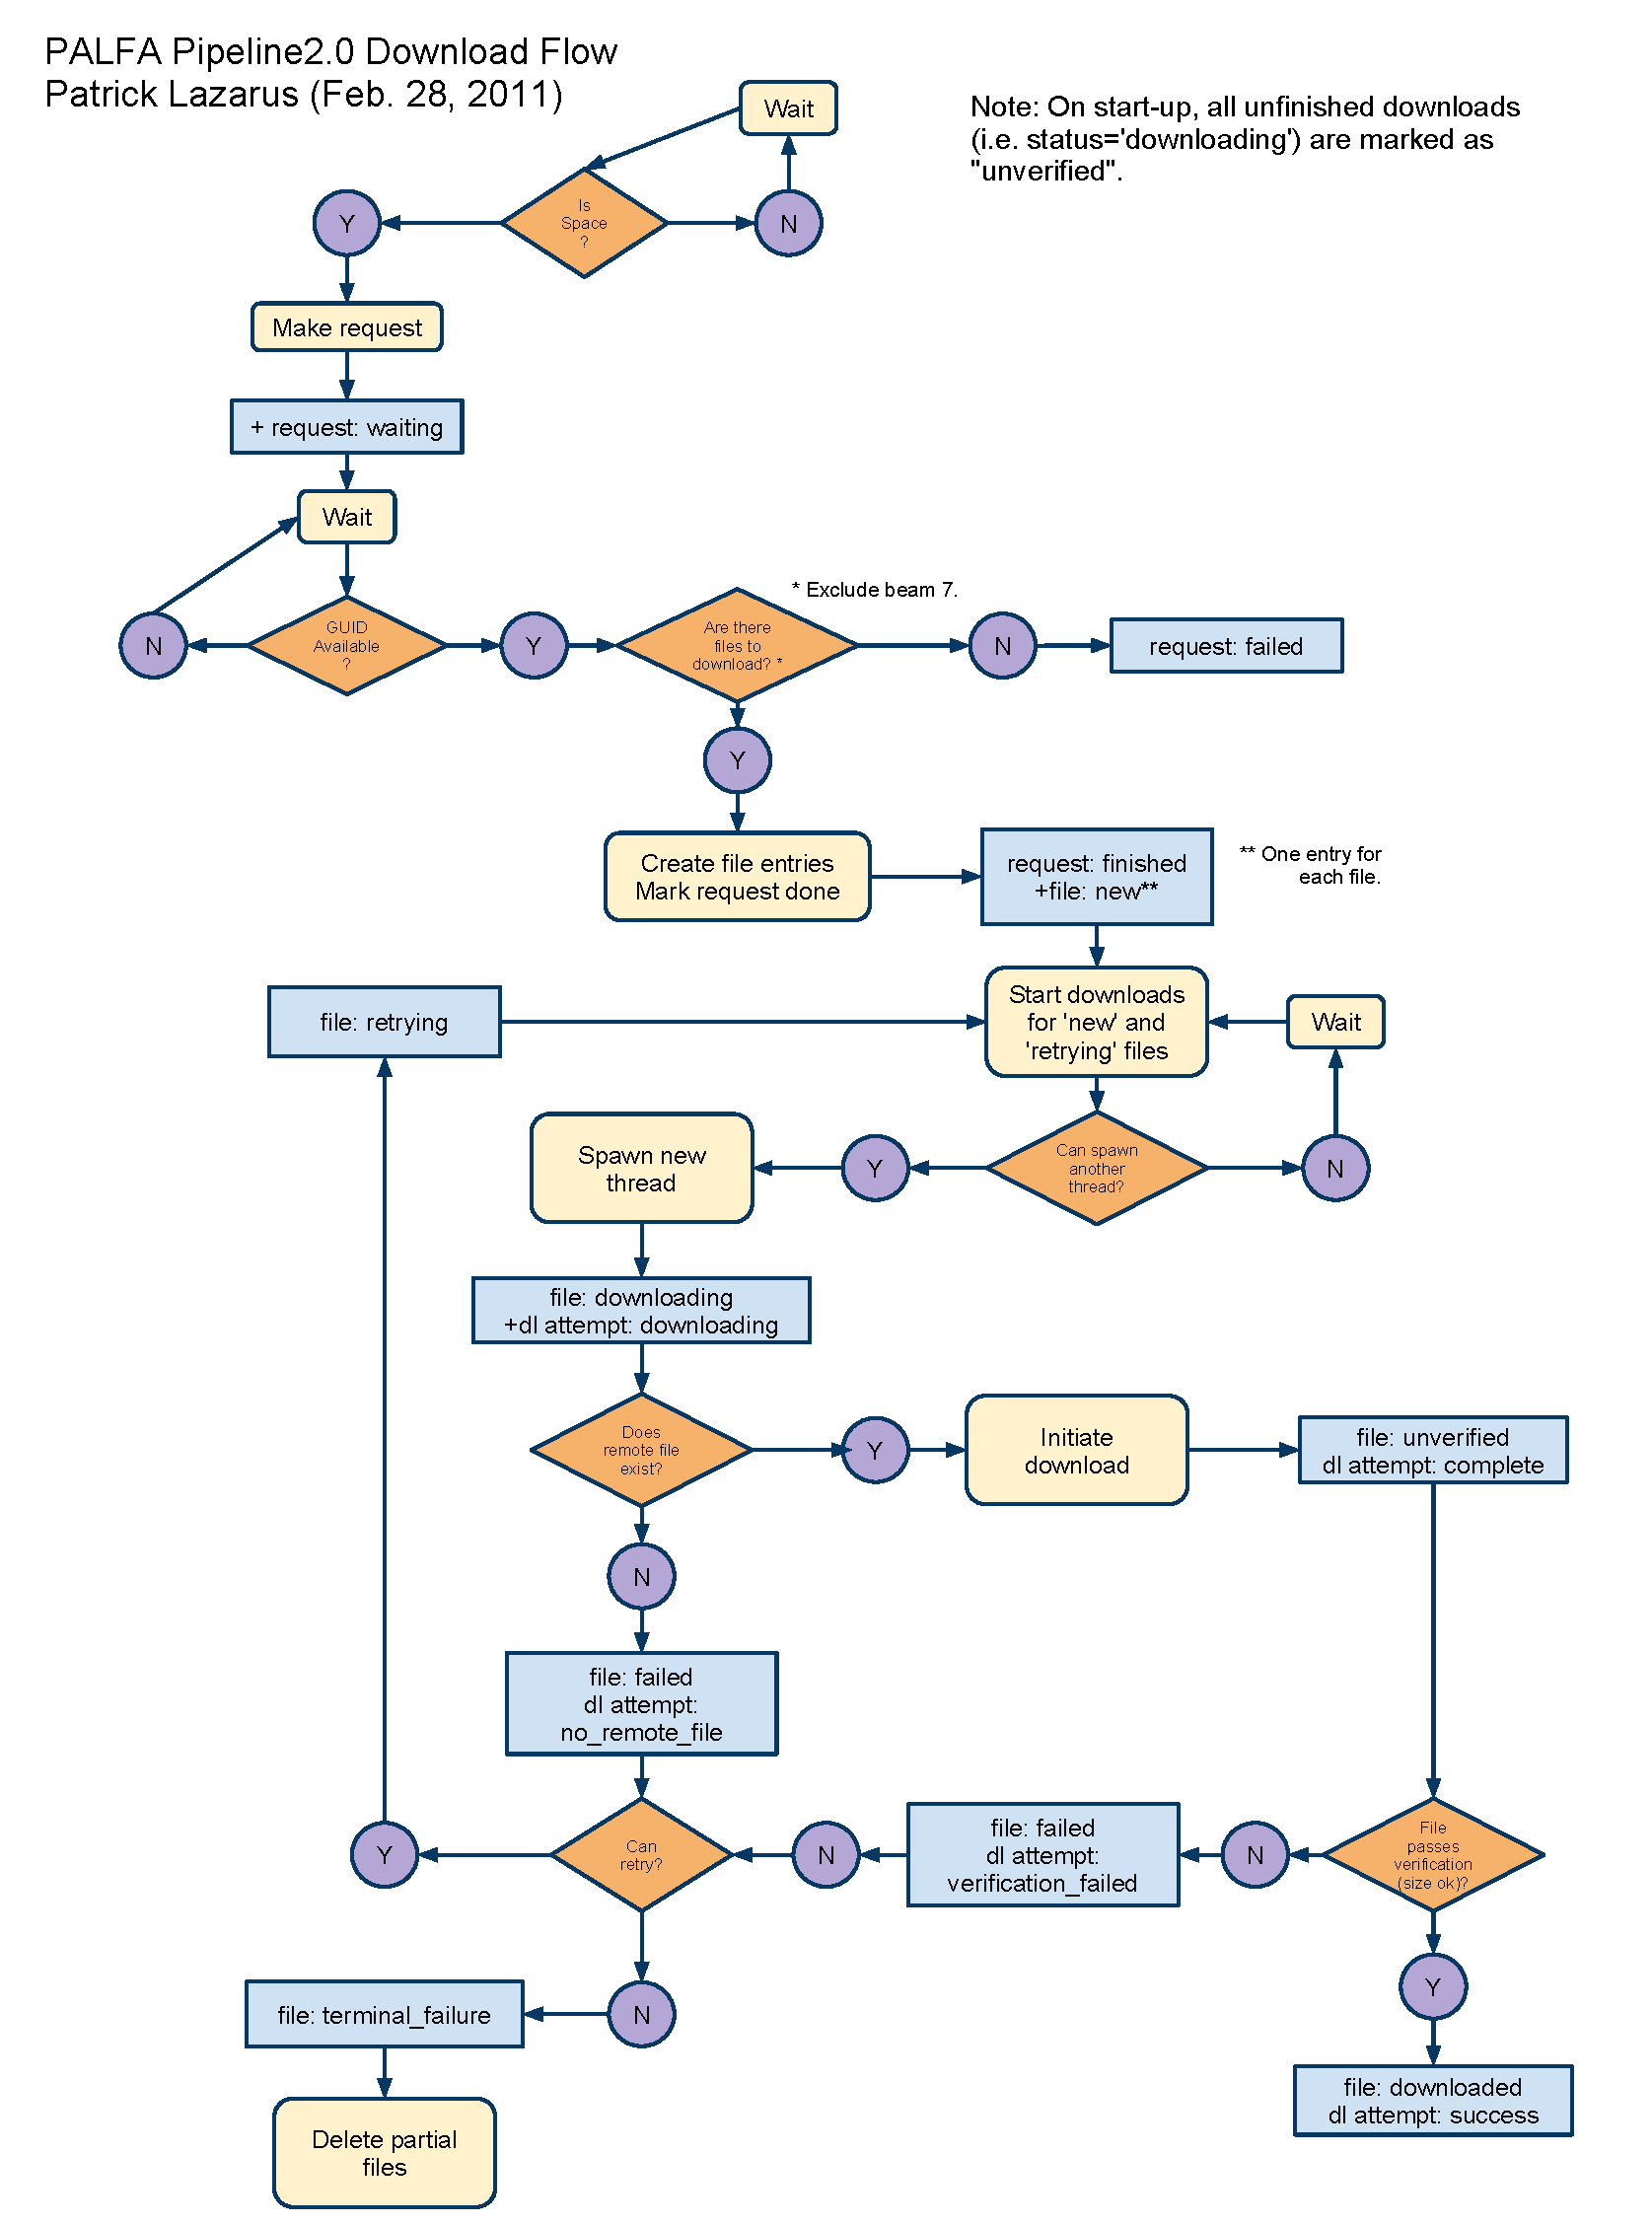
\includegraphics[scale=0.5]{./figs/ThreadedDownloadFlow.pdf}
    \caption{The flow of the download portion of the pipeline. Yellow boxes represent actions. Blue boxes represent changes in status, which are tracked in the job-tracker database. Finally, orange diamonds are decisions. \label{fig:download flow}}
\end{figure}

\begin{figure}
    \centering
    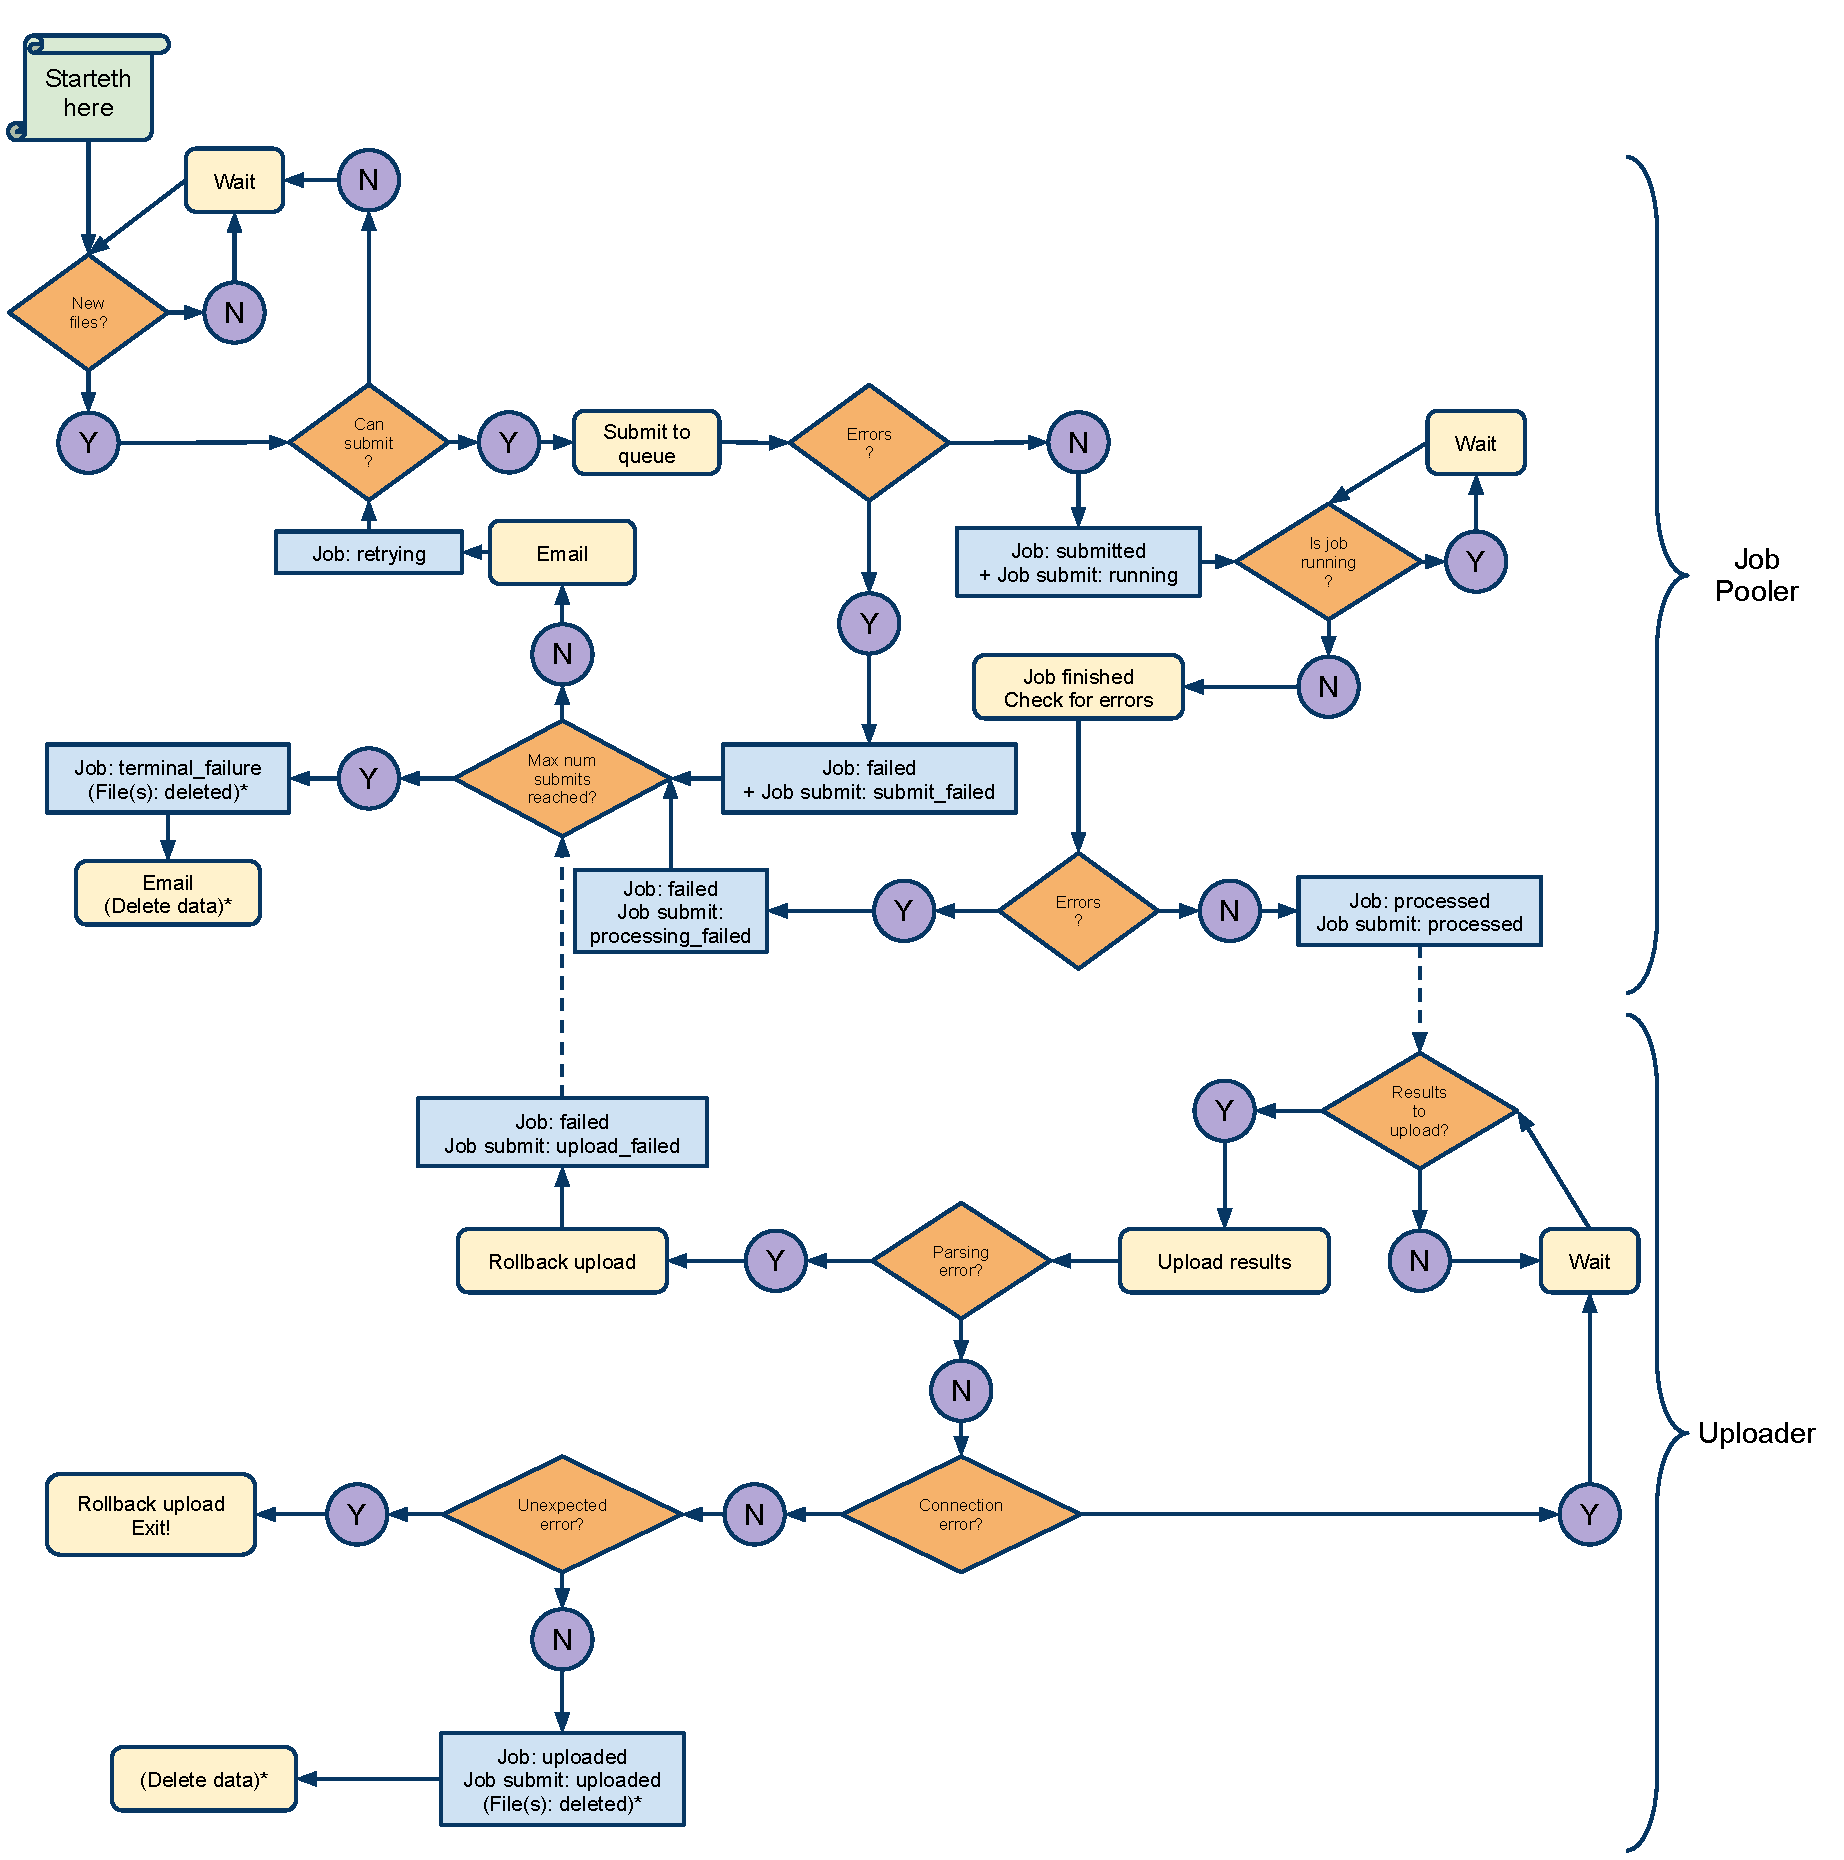
\includegraphics[scale=0.5]{./figs/JobFlow.pdf}
    \caption{The flow of the processing and results upload portions of the pipeline. Yellow boxes represent actions. Blue boxes represent changes in status, which are tracked in the job-tracker database. Finally, orange diamonds are decisions. \label{fig:job flow}}
\end{figure}


\subsection{Components}
\subsubsection{Job-tracking Database}
Each job run through the pipeline passes through multiple stages before it is completed. To track the state of each job, and log its history a SQLite3 database is used. The database is simply a (readable/writable) binary file formatted according to the SQLite3 format. The database file can be access using SQL statements using python's sqlite3 module, which is part of python's standard library, as of python version 2.5.

Relevant links:
\begin{itemize}
    \item http://docs.python.org/library/sqlite3.html
    \item http://www.sqlite.org/
\end{itemize}

The job-tracker database governs all aspects of the pipeline. It maintains lists of requests for data, downloads, jobs, files associated with each job, processing attempts, and upload attempts.

Details for each table in the database are presented in Section \ref{sec:dbdetails}.

\subsubsection{Downloader}
The downloader issues requests for PALFA data using a web service hosted at Cornell University, where the PALFA data archive is located. The ``restore'' service returns a unique identifier, which can be used to check when the requested data files are ready to be transfered using the ``location'' service. When files are ready for download entries are added to the job-tracker database for each file. The downloader then transfers the files using FTP. Downloads are threaded.

\subsubsection{Job Pooler}
The job pooler manages the data analysis stage of the pipeline by collecting data files and submitting them to compute resources available. When jobs are finished the job pooler checks for errors. If there are none the jobs are marked as ``processed''. If errors occurred during processing the job may be retried. A user-defined configuration limits the number of processing attempts before a job is aborted. In the case of aborted jobs, the data files may be deleted allowing for new files to be fetched.

\subsubsection{Uploader}
The uploader parses the data products from data analysis that terminated with no errors. The upload consists of three parts: the header (metadata about the observation), the pulsar candidates, and diagnostics about the analysis. After results are uploaded, they are retrieved from the database and compared with the results on-disk. If no errors are encountered and the database results match the on-disk results, the uploader commits the database transaction, and marks the job as ``uploaded'' and the raw data files are removed from disk to make room for new files to be downloaded.

\paragraph{Headers}
The headers contain information about the observation and data files, such as: observation date, integration time, sky position, observing band, sample time, etc.

\paragraph{Candidates}
For each periodicity candidate folded during data analysis an entry is inserted into the database. Each entry contains the candidate's period, frequency, dispersion measure, significance, etc.

In addition to candidate information two binary objects are stored in the common database:
\begin{itemize}
    \item \textit{Prepfold plot} \hfill \\
        A PNG version of the standard diagnostic plot produced by \texttt{prepfold} for the candidate.
    \item \textit{PFD binary} \hfill \\
        The binary data produced by \texttt{prepfold}. This binary file can be used to compute ratings, which are useful when querying the common database to find good pulsar candidates, or as input to artificial intelligences.
\end{itemize}

\paragraph{Diagnostics}
Diagnostics stored in the common database are split into two types: Numeric values and binary data. Some of the ``binary data" diagnostics are actually plain text files.

The following per-beam diagnostics are uploaded to the common database:
\begin{itemize}
    \item \textit{RFI mask percentage} (Numeric value) \hfill \\
        Percentage of data masked due to RFI.

    \item \textit{Num cands folded} (Numeric Value) \hfill \\
        The number of candidates folded.

    \item \textit{Num cands produced} (Numeric Value) \hfill \\
        The total number of candidates produced, including those with sigma lower than the folding threshold.

    \item \textit{Min sigma folded} (Numeric value) \hfill \\
        The smallest sigma value of all folded candidates from this beam.

    \item \textit{Num cands above threshold} (Numeric value) \hfill \\
        The number of candidates produced (but not necessarily folded) that are above the desired sigma threshold.
    
    \item \textit{RFIfind png} (Binary data) \hfill \\
        Output image produced by rfifind in png format.

    \item \textit{Accelcands list} (Binary data) \hfill \\
        The combined and sifted list of candidates produced by accelsearch.
    
    \item \textit{Zaplist used} (Binary data) \hfill \\
        The list of frequencies and ranges zapped from the power spectrum before searching this beam.
\end{itemize}

\subsection{Objects Tracked}
\paragraph{Restores}

\paragraph{Downloads}

\paragraph{Jobs}

\paragraph{Uploads}


\section{Reference}
\subsection{Database Configuration}
\label{sec:dbconf}
UnixODBC and FreeTDS need to be properly configured to be able to connect to the common database. The following configuration files are required (at McGill). These files can be placed in your home area. It is also possible to put these configurations in a system configuration directory so all users will have access to them automatically. System-wide configuration files at McGill are \texttt{/etc/odbc.ini} and \texttt{/etc/freetds/freetds.conf}.

Be sure to increase the \texttt{text size} in \texttt{freetds.conf}. It is the maximum size for binary files that can be transfered. The value below ($\sim$ 16 MB) should be sufficient for the pipeline.

\paragraph{\texttt{.obdc.ini}}
\begin{verbatim}
    [ODBC Data Sources]
    FreeTDSDSN = FreeTDS
    MySQLDSN   = MySQL

    [FreeTDSDSN]
    Driver          = /usr/lib/odbc/libtdsodbc.so
    Servername      = Cornell
    Description     = FreeTDS
    Database        = palfa-common

    [MySQLDSN]
    Driver          = /usr/lib/odbc/libmyodbc.so
    Description     = MySQL

    [Default]
    Driver          = /usr/lib/odbc/libtdsodbc.so
\end{verbatim}

\paragraph{\texttt{.freetds.conf}}
\begin{verbatim}
    #   $Id: freetds.conf,v 1.12 2007/12/25 06:02:36 jklowden Exp $
    #
    # This file is installed by FreeTDS if no file by the same 
    # name is found in the installation directory.  
    #
    # For information about the layout of this file and its settings, 
    # see the freetds.conf manpage "man freetds.conf".  

    # Global settings are overridden by those in a database
    # server specific section
    [global]
            # TDS protocol version
    ;       tds version = 4.2

            # Whether to write a TDSDUMP file for diagnostic purposes
            # (setting this to /tmp is insecure on a multi-user system)
    ;       dump file = /tmp/freetds.log
    ;       debug flags = 0xffff

            # Command and connection timeouts
    ;       timeout = 10
    ;       connect timeout = 10
            
            # If you get out-of-memory errors, it may mean that your client
            # is trying to allocate a huge buffer for a TEXT field.  
            # Try setting 'text size' to a more reasonable limit 
            text size = 16777215

    # A typical Sybase server
    [egServer50]
            host = symachine.domain.com
            port = 5000
            tds version = 5.0

    # A typical Microsoft server
    [egServer70]
            host = ntmachine.domain.com
            port = 1433
            tds version = 7.0

    [Cornell]
            host = arecibosql.tc.cornell.edu
            port = 1433
\end{verbatim}

\subsection{Tests}
\label{sec:tests}
The pipeline contains several tests that can be used to confirm certain tricky aspects of the pipeline are configured properly. These tests are located in \texttt{tests/}.

\begin{description}
    \item[commondb\_test.py] This script tests that connections to the common database. It also verifies that it is possible to read from the database, as well as insert entries into the database.

    \item[cornellftp\_test.py] This test confirms that it is possible to connect to the FTP server at Cornell, access information about files available, and retrieve files.

    \item[install\_test.py] This script attempts to import all python modules necessary by the pipeline. If any modules were not successfully imported they are reported to the user.

    \item[mailer\_test.py] This script attempts to send an email using the SMTP server defined in the configuration file \texttt{email.py}.

    \item[restore\_test.py] This script verifies that the pipeline can connect to the data-restore web services, make requests and check when data are available.
\end{description}

\subsection{Executables}
The pipeline has a series of executables located in the 'bin/' directory. There are two categories of executables: background scripts, and utilities.

\subsubsection{Background scripts}
The following background scripts are used to run the Downloader, Job Pooler and Uploader.
\begin{itemize}
    \item \texttt{StartDownloader.py} \hfill \\
        A script to start the downloader background process.

        usage: \texttt{StartDownloader.py}

    \item \texttt{StartJobPool.py} \hfill \\
        A script to start the job pooler background process.

        usage: \texttt{StartJobPool.py}

    \item \texttt{StartJobUploader.py} \hfill \\
        A script to start the results uploader background process.

        usage: \texttt{StartJobUploader.py}
\end{itemize}

\subsubsection{Utilities}
The following utility scripts are used to interact with the job-tracker database in a safe way. This includes creating the database, editing the entries in the database, and compiling and displaying information from the database entries.
\begin{itemize}
    \item \texttt{add\_files.py} \hfill \\
        A utility to add files from a given directory to be tracked. This is useful for tracking files that are copied over from an external disk, as opposed to downloaded by the Downloader. Note that added files will be deleted just like downloaded files.

        \textbf{usage:} \texttt{add\_files.py DIRECTORY} \\

    \item \texttt{stop\_processing\_jobs.py} \hfill \\
        Stop a job running in the queue. There are two ways to stop jobs: 1) Failing the job (i.e. the submission counts towards the job's number of retries, and 2) Removing the job (the submission doesn't count towards retries). Both possibilities are done safely, with respect to the job-tracker DB. The default is to remove the jobs (not fail).

        \textbf{usage:} \texttt{stop\_processing\_jobs.py [OPTIONS] QUEUE\_ID [QUEUE\_ID ...]} \\
        \textbf{options:} \\
            \texttt{-h, --help}  Show help message and exit. \\
            \texttt{-f, --fail}  Remove jobs from the queue and mark them as 'failed' in the job-tracker database. (Default: Remove jobs and don't mark them as'failed').

    \item \texttt{create\_database.py} \hfill \\
        Create the sqlite job-tracker database. Note that the script will do nothing if the database already exists. The location of the database is taken from the database configuration file.

        \textbf{usage:} \texttt{create\_database.py}

    \item \texttt{kill\_jobs.py} \hfill \\
        Kill a job. That is set its status as 'terminal\_failure', and clean up its datafiles (if applicable).

        \textbf{usage:} \texttt{kill\_jobs.py ID [ID ...]} \\
        \textbf{options:} \\
          \texttt{-h, --help}            Show help message and exit. \\
          \texttt{-f FILES, --file=FILES}  File belonging to a job that should be killed. \\
          \texttt{-i JOBIDS, --id=JOBIDS}  ID number of a job that should be killed.

\end{itemize}

\subsection{Generic Queue Manager Interface}
The Pipeline interacts with the system's queue manager using an abstract interface. This generic interface can be implemented with the specific queue manager installed on the system. The system-specific queue manager class must be derived from the \texttt{generic\_interface.PipelineQueueManager} class. Each of the following methods must be implemented in the derived class:

\begin{description}
    \item[submit] Submits a job to queue manager with files list and output directory. Must return a unique string identifier for the submitted job. Raises \texttt{pipeline\_utils.PipelineError} if job submission fails.

    \item[can\_submit] Return a bollean value that indicates if jobs can be submitted to the queue.
    
    \item[is\_running] Given a unique identifier for a job, must return True or False whether the job is running or not, respectively.

    \item[delete] Given a unique identifier for a job, remove the corresponding job from the queue. Raises \texttt{pipeline\_utils.PipelineError} if job removal isn't successful.

    \item[status] Return the status of the queue as a tuple containing the number of jobs running and the number of jobs queued.

    \item[had\_errors] Given a unique identifier for a job, return True, or False whether the job terminated with an error, or not, respectively.

    \item[get\_errors] Given a unique identifier for a job, return the contents of the error log. If there were not errors return an empty string.
\end{description}


\subsection{Configurations}
\label{sec:configs}

The pipeline requires a series of configurations to be set in order to run. The configurations for different aspects of the pipeline are divided into the different files. The configuration files can be found in the pipeline's lib/python/config/ directory.

A sanity check of configurations is performed each time a configuration file is imported. If there are errors (e.g. a setting isn't provided, a directory doesn't exist, etc.) a message is printed to the terminal, and an exception is raised causing the program to exit. It is possible to run the check the sanity of a configuration file by running it. For example, checking the sanity of \texttt{basic.py}:

\texttt{python basic.py}

If the settings are sane there will be no error message is output. \textit{NOTE: it may be necessary to check the sanity of the processing configurations on the worker nodes.}

Each of required settings in each of the configration files are listed below:

\subsubsection{basic.py}
Basic pipeline parameters are found in \texttt{basic.py}.

\begin{description}
    \item[institution] Institution where the pipeline is being run. This is the value that will get reported in the common database.
    \item[pipeline] The type of pipeline being run. This should be left as ``PRESTO''.
    \item[survey] The name of the survey. This should be left as ``PALFA2.0''.
    \item[pipelinedir] The path of the base directory containing the pipeline2.0 code.
    \item[psrfits\_utilsdir] The path of the directory containing the installation of \texttt{psrfits\_utils} that is used by the pipeline.
    \item[delete\_rawdata] A boolean value that determines if raw data is deleted when results for a job are successfully uploaded to the common DB, or if the maximum number of attempts for a job is reached. \textit{Set this value to False if you do not want the local copy of your data deleted.}
    \item[coords\_table] The path to the \texttt{PALFA\_coords\_table.txt} file, which contains correct coordinates for WAPP data files.
    \item[log\_dir] The path of the directory where log files are stored.
    \item[qsublog\_dir] The path where stderr streams from processing jobs are sent.
\end{description}

\subsubsection{background.py}
General settings for the three background scripts are found in \texttt{background.py}

\begin{description}
    \item[screen\_output] A boolean value that should be set to True if you want log information copied to the terminal.
    \item[jobtracker\_db] The path to the SQLite job-tracker database.
    \item[sleep] The number of seconds to sleep between iterations of the background scripts' loops.
\end{description}


\subsubsection{commondb.py}
The information needed to connect to the common database is in \texttt{commondb.py}.

\begin{description}
    \item[username] The common database user name.
    \item[password] The password used to access the common database.
    \item[host] The computer through which a connection to the common database will be established. This should be left at ``arecibosql.tc.cornell.edu''.
\end{description}


\subsubsection{download.py}
Informatation necessary to connect to the FTP server at Cornell and use the data-restore web applications are set in \texttt{download.py}, so are settings for controlling the behaviour of the downloader.

\begin{description}
    \item[api\_service\_url] This is the URL of the data-restore web apps. This should be set to ``http://arecibo.tc.cornell.edu/palfadataapi/dataflow.asmx''.
    \item[api\_username] This is your user name used to connect to the data-restore web apps.
    \item[api\_password] This is the password for connecting to the data-restore web apps.
    \item[ftp\_host] This is the name of the FTP server at Cornell. It should be left at ``arecibo.tc.cornell.edu''.
    \item[ftp\_port] This is the port to use for FTP. It should be 31001.
    \item[ftp\_username] This is the user name to connect when FTP'ing. Currently all downloaders are using a shared account, so this should have the value ``palfadata''.
    \item[ftp\_password] This is the password of the FTP account.
    \item[temp] This is the directory where data are downloaded to.
    \item[space\_to\_use] This is the space available for downloaded files, measured in bytes.
    \item[numdownloads] This is the number of downloads that can be run in parallel.
    \item[numrestored] This is the maximum number of files requested + number of files to be downloaded at any given time.
    \item[numretries] This is the number of times a download will be attempted before giving up and moving on to another file.
    \item[use\_lftp] A boolean value. If True download files using a system call to the program \texttt{lftp}, otherwise use the pipeline's FTP client based on M2Crypto and ftplib.
\end{description}


\subsubsection{email.py}
The pipeline can be configured to send emails when failures occur. The relevant settings are in \texttt{email.py}.

\begin{description}
    \item[enabled] A boolean value that enables mailing. If False emails will not be sent.
    \item[smtp\_host] Emails are sent using the Simple Mail Transfer Protocol (SMTP). This is the host of the SMTP server to use. If set to \texttt{None} the localhost will be used as a SMTP server to send the emails.
    \item[smtp\_port] The emailer connects to the SMTP server using this port. Either 25 or 587 should work, possibly both.
    \item[smtp\_username] The user account to connect to the SMTP server.
    \item[smtp\_password] The password to connect to the SMTP server.
    \item[smtp\_usetls] A boolean value that determines whether or not Transport Layer Security (TLS) should be used. Some SMTP servers don't support it.
    \item[smtp\_usessl] A boolean value that determines whether or not Secure Sockets Layer (SSL) should be used. This functionality requires python2.6 or newer.
    \item[smtp\_login] A boolean value that determines if username/passsword are used to log into the SMTP server.
    \item[recipient] The email address that will be sent notifications.
    \item[send\_on\_failures] A boolean value that determines if emails should be sent when a job fails.
    \item[send\_on\_terminal\_failures] A boolean value that determines if emails should be sent on terminal failures (i.e. job will not be re-tried). Note: if ``\texttt{send\_on\_failures}'' is True emails will be sent on terminal failures regardless of the value of ``\texttt{send\_on\_terminal\_failures}.
\end{description}


\subsubsection{jobpooler.py}
The setting that determine the behaviour of the Job Pooler are in \texttt{jobpooler.py}.

\begin{description}
    \item[base\_results\_directory] The path of where results from processing are stored. Note: the processing of each data set is in a separate subdirectory.
    \item[max\_jobs\_running] The maximum number of jobs running at any given time.
    \item[max\_jobs\_queue] The maximum number of jobs that are allowed to be queued at any given time. This must be at least 1, otherwise the Job Pooler will not submit jobs for fear of them being queued.
    \item[max\_attempts] The maximum number of times a job is submitted before being abandoned.
    \item[queue\_manager] An instance of a sub-class of \texttt{PipelineQueueManager}. This is the interface between the pipeline and the queue manager.
\end{description}

\subsubsection{processing.py}
Setting required during processing (i.e. on the worker nodes) are provided in \texttt{processing.py}.

\begin{description}
    \item[base\_working\_directory] The directory on the worker node where temporary working and results directories will be placed.
    \item[default\_zaplist] The path of the zaplist to use when no MJD-specific zaplist can be found.
    \item[zaplistdir] The directory containing MJD-specific zaplists.
\end{description}


\subsubsection{searching.py}
The search parameters of the pipeline are located in \texttt{searching.py}. To ensure searching is done uniformly across all processing sites most of these values shouldn't be modified.

\begin{description}
    \item[use\_subbands] A boolean value that determines if we'll dedisperse and fold using subbands. In general, it is a very good idea to use them if there is enough scratch space on the machines that are processing ($\sim$30GB/beam processed).
    \item[fold\_rawdata] A boolean value that determines if folding should be done from the raw FITS files (as opposed to subbands or dedispersed FITS files).
    \item[datatype\_flag] This is the flag provided to PRESTO programs to indicated the data type. This should be ``-psrfits''.
    \item[rfifind\_chunk\_time] The duration of each chunk in \texttt{rfifind}.
    \item[singlepulse\_threshold] The threshold SNR for singlepulse candidate determination.
    \item[singlepulse\_plot\_SNR] The threshold SNR for displaying singlepulse candidates on plots.
    \item[singlepulse\_maxwidth] The maximum pulse width (in seconds) for singlepulse searching.
    \item[to\_prepfold\_sigma] The minimum incoherent sum significance required to fold a candidate.
    \item[max\_cands\_to\_fold] The maximum number of candidates to fold per beam.
    \item[numhits\_to\_fold] The minimum number of DMs at which a periodicity must be found to be folded.
    \item[low\_DM\_cutoff] The lowest DM to consider when choosing candidates to fold.
    \item[lo\_accel\_numharm] The maximum number of harmonics to sum in low acceleration searching.
    \item[lo\_accel\_sigma] The minimum gaussian significance threshold in low acceleration searching.
    \item[lo\_accel\_zmax] The maximum z-value (in bins) used in low acceleration searching.
    \item[lo\_accel\_flo] The maximum frequency searched in low acceleration searching.
    \item[hi\_accel\_numharm] The maximum number of harmonics to sum in high acceleration searching.
    \item[hi\_accel\_sigma] The minimum gaussian significance threshold in high acceleration searching.
    \item[hi\_accel\_zmax] The maximum z-value (in bins) used in high acceleration searching.
    \item[hi\_accel\_flo] The maximum frequency searched in high acceleration searching.
    \item[low\_T\_to\_search] The shortest observation that will be searched (in seconds).
    \item[base\_tmp\_dir] The path where the temporary working directory should be created. This could be /dev/shm, for example. If /dev/shm doesn't exist, or is too small, this path could simply be another path in the scratch area of the worker node.
    \item[sifting\_sigma\_threshold] The minimum incoherent power sigma to consider when sifting candidates. This should be left at \texttt{to\_prepfold\_sigma}$-$1.0.
    \item[sifting\_c\_pow\_threshold] The coherent power threshold used when sifting.
    \item[sifting\_r\_err] The Fourier bin tolerance to consider two candidates as being at the same frequency.
    \item[sifting\_short\_period] The shortest candidate period to consider (in seconds).
    \item[sifting\_long\_period] The longest cndidate period to consider (in seconds).
    \item[sifting\_harm\_pow\_cutoff] The power required in at least one harmonic.
\end{description}
    

\subsubsection{upload.py}
Configurations used by the uploader are set in \texttt{upload.py}.

\begin{description}
    \item[version\_num] The version number of the current version of the pipeline (including versions of \texttt{PRESTO} and \texttt{psrfits\_utils}). The preferred format is:
    
    \texttt{PRESTO:\{git-hash\};PIPELINE:\{git-hash\};PSRFITS\_UTILS\{git-hash\}}. 
    
    It is \textbf{strongly} recommended that the git-hash values are retrieved dynamically, so they are always up-to date. However, if this is not possible you are able to hard code values of the git-hashes, but they should be changed every time the versions of the software used are modified.
\end{description}


\subsection{Job-Tracker Database Details}
\label{sec:dbdetails}

The job-tracker database is an SQL lite database, which is simply a binary file stored on disk. The database file is accessed using python's sqlite3 module. This module is part of python's standard library as of python2.5. 

When setting up the job-tracker database be advised that it is possible there are some issues with accessing the database file over NFS (for more details see item 5 at http://www.sqlite.org/faq.html).

The job-tracker database contains six tables: \texttt{requests}, \texttt{files}, \texttt{download\_attempts}, \texttt{jobs}, \texttt{job\_files}, and \texttt{job\_submits}. Each of these tables is meant to track a particular object (e.g. jobs), or events (e.g. job submissions to the queue).

A description of each database table will now be presented:

\subsubsection{\texttt{requests}}
The \texttt{requests} table tracks requests for data restores. An entry in the table is inserted when a request is made. Each entry contains the following data:
\begin{description}
    \item[id] (UNIQUE INTEGER) A unique identifier, automatically assigned by the database upon creation of an entry.
    \item[size] (INTEGER) Total size of the files restored, in bytes.
    \item[guid] (TEXT) A globally unique identifier for the restore. This serves as the directory name on the FTP server where the restored files will be placed.
    \item[status] (TEXT) The current status of the request.
    \item[details] (TEXT) Details about the request.
    \item[created\_at] (TEXT) Date and time when the request entry was created.
    \item[updated\_at] (TEXT) Date and time when the request entry was last updated.
\end{description}

\subsubsection{files}
The \texttt{files} table tracks each file available to the pipeline. A separate entry is inserted for each file. Each entry contains the following data:

\begin{description}
    \item[id] (UNIQUE INTEGER)  A unique identifier, automatically assigned by the database upon creation of an entry.
    \item[filename] (TEXT) The name of the file.
    \item[remote\_filename] (TEXT) The name and path of the downloaded file on the FTP server.
    \item[request\_id] (INTEGER) The identifier of the entry in the \texttt{requests} table that restored this file.
    \item[status] (TEXT) The current status of the file.
    \item[details] (TEXT) Details about the file.
    \item[created\_at] (TEXT) Date and time when the file entry was created.
    \item[updated\_at] (TEXT) Date and time when the file entry was last updated.
\end{description}

\subsubsection{download\_attempts}
Every time one an attempt to download one of the files listed in the \texttt{files} table an entry is created in the \texttt{download\_attempts} table. Each download attempt entry has the following data:

\begin{description}
    \item[id] (UNIQUE INTEGER)  A unique identifier, automatically assigned by the database upon creation of an entry.
    \item[request\_id] (INTEGER) The identifier of the entry in the \texttt{files} table that this download attempt corresponds to.
    \item[status] (TEXT) The current status of the download attempt.
    \item[details] (TEXT) Details about the current status of the download attempt.
    \item[created\_at] (TEXT) Date and time when the download attempt entry was created.
    \item[updated\_at] (TEXT) Date and time when the download attempt entry was last updated.
\end{description}

\subsubsection{jobs}
Each beam-worth of data gets submitted to be processed as a single job. These jobs are tracked in the \texttt{jobs} table, and have the following data:

\begin{description}
    \item[id] (UNIQUE INTEGER)  A unique identifier, automatically assigned by the database upon creation of an entry.
    \item[status] (TEXT) The current status of the job.
    \item[details] (TEXT) Details about the current status of the job.
    \item[created\_at] (TEXT) Date and time when the job entry was created.
    \item[updated\_at] (TEXT) Date and time when the job entry was last updated.
\end{description}

\subsubsection{job\_files}
Because a job can have multiple files a mapping between jobs and files is required. The \texttt{job\_files} table serves this purpose. Each row in the table has the following data:

\begin{description}
    \item[id] (UNIQUE INTEGER)  A unique identifier, automatically assigned by the database upon creation of an entry.
    \item[file\_id] (INTEGER) The indentifier of an entry in the \texttt{files} table.
    \item[job\_id] (INTEGER) The identifier of an entry in the \texttt{jobs} table that the file referred to by \texttt{file\_id} belongs to.
    \item[created\_at] (TEXT) Date and time when the entry was created.
    \item[updated\_at] (TEXT) Date and time when the entry was last updated.
\end{description}

\subsubsection{job\_submits}
Each submission of a job to the queue to be processed is tracked in the \texttt{job\_submits} table. Each job submission has the following information:

\begin{description}
    \item[id] (UNIQUE INTEGER)  A unique identifier, automatically assigned by the database upon creation of an entry.
    \item[queue\_id] (TEXT) The unique identifier assigned to the job by the queue manager when it is submitted. This identified is used to check if the submission is still being processed.
    \item[job\_id] (INTEGER) The identifier of the job (from the \texttt{jobs} table) that was submitted for processing.
    \item[output\_dir] (TEXT) The directory where the results of processing will be output.
    \item[status] (TEXT) The current status of the job.
    \item[details] (TEXT) Details about the current status of the job.
    \item[created\_at] (TEXT) Date and time when the entry was created.
    \item[updated\_at] (TEXT) Date and time when the entry was last updated.
\end{description}

\end{document}
